\documentclass[12pt]{article}
\usepackage{amsfonts, epsfig}

\usepackage{graphicx}
\usepackage{fancyhdr}
\pagestyle{fancy}
\lfoot{\texttt{github.com/conorhoughton/COMS30127}}
\lhead{Computation Neuroscience - 03.5\_cerebellum - Conor}
\rhead{\thepage}
\cfoot{}

\usepackage{graphicx}
\usepackage{listings}

\usepackage{tikz}

\usepackage{pgf}
\usepackage[utf8]{inputenc}
\usetikzlibrary{arrows,automata}
\usetikzlibrary{positioning}


\tikzset{
    state/.style={
           rectangle,
           rounded corners,
           draw=black, very thick,
           inner sep=2pt,
           text centered,
           },
}
\tikzset{
    on/.style={
           circle,
           draw=red, very thick,
           inner sep=2pt,
           fill=red!25,
           },
}


\tikzset{
    off/.style={
           circle,
           draw=blue, very thick,
           inner sep=2pt,
           text centered,
           },
}



\tikzset{
    neuron/.style={
           rectangle,
           rounded corners,
           draw=black, very thick,
           inner sep=2pt,
           text centered,
           },
}



\tikzset{
    area/.style={
           rectangle,
           draw=black, very thick,
           inner sep=2pt,
           text centered,
           },
}


\tikzset{
    gc/.style={
           rectangle,
           rounded corners,
           draw=red, very thick,
           inner sep=2pt,
           text centered,
           },
}


\tikzset{
    inh/.style={
           rectangle,
           rounded corners,
           draw=blue, very thick,
           inner sep=2pt,
           text centered,
           },
}



\tikzset{
    io/.style={
           rectangle,
           draw=green, very thick,
           inner sep=2pt,
           text centered,
           },
}



\usepackage{ifthen}
\newboolean{nopics}
\setboolean{nopics}{true}


\begin{document}

\subsection*{The cerebellum as a perceptron}

The cerebellum has a number of striking features; it has a more
stereotypical structure than most brain area and this structure is
conserved across species. It also has one of the brain's largest cells,
the Purkinje cell, and its most numerous, the granule cell.

\begin{figure}
  \ifthenelse{\boolean{nopics}}
             {{\textsl{This is a drawning of a cell, it has an extremely complicated, imagine the road network for a vast unplanned housing development with some larger roads and from them smaller roads all leading to one place, in this case the soma. The dentritic arbour is roughly square, an axon extends down from the soma.}}}
             {
  \begin{center}
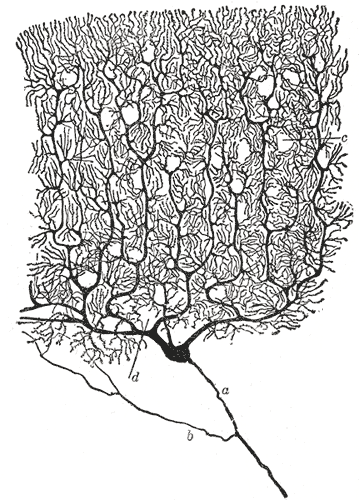
\includegraphics[width=7cm]{Purkinje_cell_by_Cajal.png}
  \end{center}
  }
\caption{A drawing by Santiago Ram\'{o}n y Cajal of a Purkinje cell. [Picture taken from \texttt{http://en.wikipedia.org/wiki/Golgi's\_method}]\label{fig:PC}}
\end{figure}

Purkinje cells have a distinctive structure with a huge, highly
branched, but flat dendritic arbor, see Fig.~\ref{fig:PC}; this allows
an extensive connectivity with each Purkinje cell receiving inputs
from around 100,000 other cells. In the cerebellum the Purkinje cell
are lined up like pages in a book, with their arbors lying in parallel
planes. They receive two excitatory inputs, weak inputs from parallel
fibres, axons that run perpendicular to the planes of the Purkinje
cell dendritic arbors, and a strong input from a climbing fibre, a
single axon which winds around the Purkinje cell and makes multiple
contacts with it, see Fig.~\ref{fig:cerebellum}.

\begin{figure}
  \ifthenelse{\boolean{nopics}} {{\textsl{In this diagram the Purkinje
        cells are shown lined up, their dendritic arbours lying flat
        to each other, perpendicular to them the parallel fibres,
        these are shown running through the different arbours, they originate at small cells labelled granule cells. The climbing fibres are also shown, each one winding around the soma and proximal dendrites of one Purkinje cell.}}}
  {
  \begin{center}
    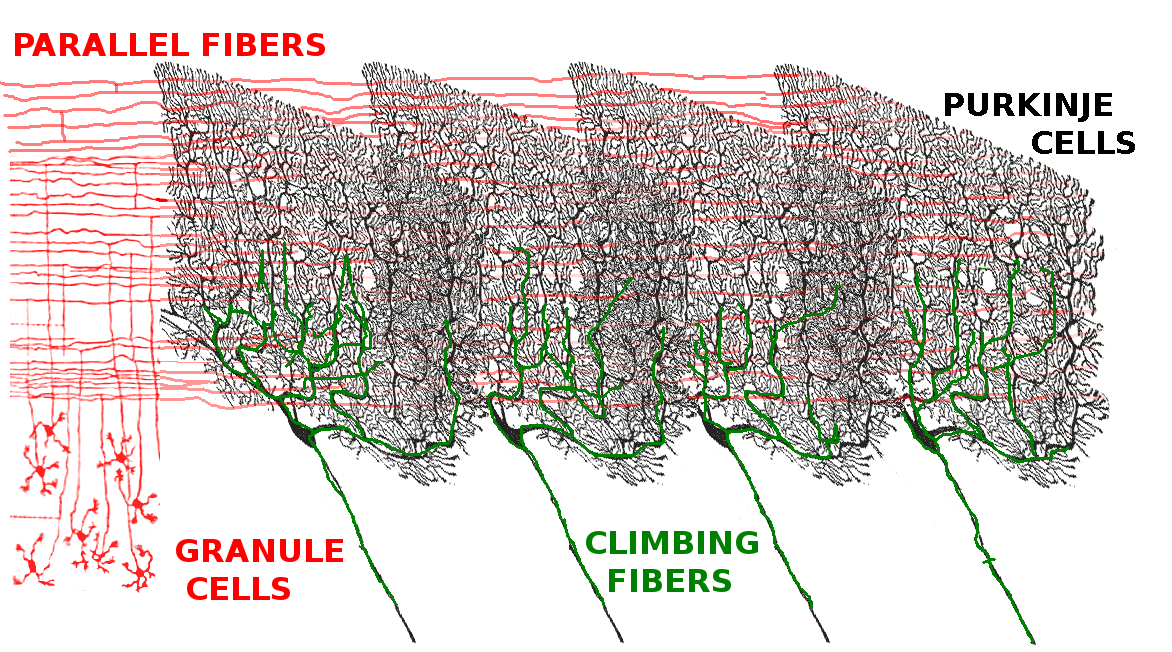
\includegraphics[width=11cm]{cerebellum.png}
  \end{center}
  }
\caption{A cartoon of the cerebellar circuitry. A vertical axon rises
  from each granule cells, splits once and then extends horizontally
  in two directions making connections with multiple Purkinje
  cells. Each Purkinje cell has its own climbing fiber which winds up
  around it.\label{fig:cerebellum}}
\end{figure}

Another peculiarity is that the Purkinje cell has different responses
to different inputs; in response to multiple weak inputs from the
parallel fibers it fires a normal sort of spike, called in this
context a \textsl{simple spike}; in response to single spike from the
climbing fiber is fires a special spike, called a \textsl{complex
  spike}, with a leading spike, a number of small \lq{}spikelets\rq{}
and a sustained after-period of depolarization; this is illustrated in
Fig.~\ref{fig:spikes}.

\begin{figure}
  \ifthenelse{\boolean{nopics}}
             {{\textsl{The simple spikes look like any other spike, but the complex spike as two small spikelets after it and then a gap before spiking resumes.
             }}}
             {
  \begin{center}
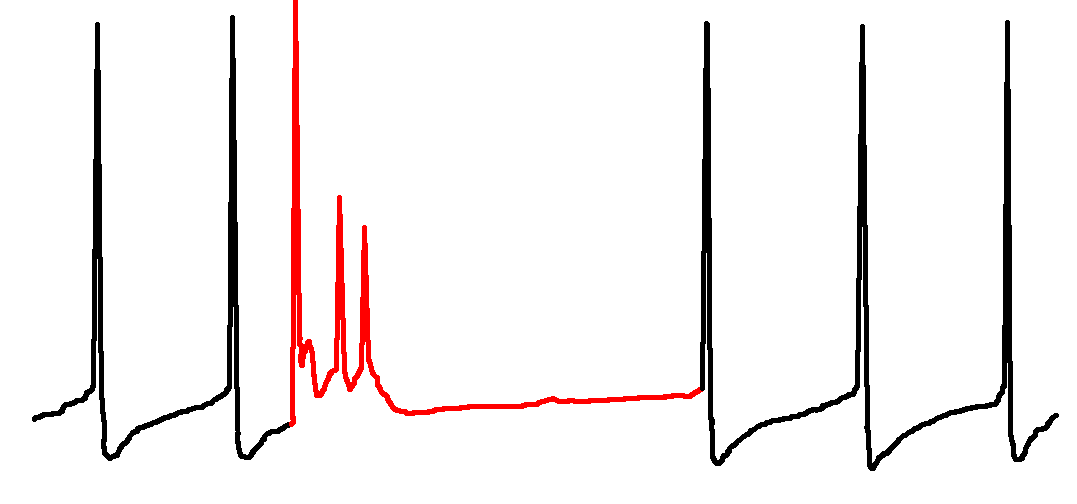
\includegraphics[width=8.cm]{complex_spike.png}
  \end{center}
  }
\caption{A complex spike. This drawing shows simple spikes in black
  and a complex spike in red. The complex spike is followed by a long
  refractory period during which spiking is not possible. This is a
  sketch, not an actual recording, but a typical time scale would have
  this refractory period 50 ms long.\label{fig:spikes}}
\end{figure}

It is still unclear exactly what the cerebellum does; what is known is
that it is important for actions, fine motor control and
proprioception; problems with the cerebellum are associated with
ataxia, loss of fine motor control, poor motor learning and poor
balance. There is a specific gait associated with cerebellar damage,
one that exhibits a certain self-consciousness or vigilance is
required for movement. According to most ideas about cerebellar
function it is required for the calculation of fine motor signals
\cite{Albus1971a}, or for predicting the sensory or proprioceptive
consequences of motor actions \cite{GaoEtAl1996a}; it is believed it
encodes forward and backwards models of movement so that it predicts
the consequences of motor commands, or calculates the motor command
that will a particular movement.

Whatever exactly it does, it is widely believed, in accordance with
the Marr-Albus model \cite{Marr1969a,Albus1971a}, that the connections
from parallel fibers to Purkinje cells acts as a perceptron. Thus, if
$y$ is the output of the Purkinje cell and, in this simple model,
taking into account the fact Purkinje cells are inhibitory
\begin{equation}
y=-\sum{w_ix_i}
\end{equation}
where the $x_i$s are the activities in the parallel fibers and $w_i$
is the strength of the synapse from the $i$th parallel fiber to the
Purkinje cell. The idea in the Marr-Albus model is that the climbing
fiber carries the error signal $d-y$ making the cerebellum an example
of supervised learning.

\begin{thebibliography}{10}

\bibitem{Albus1971a}
Albus, JS. (1971) A theory of cerebellar function. 
\newblock Mathematical Biosciences 10: 25--61.


\bibitem{GaoEtAl1996a}
Gao J-H, Parsons LM, Bower JM, Xiong J, Li J and Fox PT (1996) Cerebellum implicated in sensory acquisition and discrimination rather than motor control.
\newblock Science 272: 545--7. 

\bibitem{Marr1969a}
Marr, D (1969) A theory of cerebellar cortex.
\newblock Journal of Physiology 202: 437--70.


\end{thebibliography}

\end{document}

